\section{Results}
\label{sec:results}

This section presents our empirical findings across four primary metrics: classification accuracy, compiled model size, hardware latency, and peak runtime memory consumption. Direct analytical interpretations of these metrics are integrated into each respective results section, followed by a consolidated discussion of architectural trade-offs, system constraints, and broader structural limitations.

\subsection{Model Accuracy and Storage Fingerprint}

We first validated the baseline classification performance on a development PC using our custom PyTorch implementation of the Mamba block. Training achieved validation accuracies of 98.6\% on the Human Activity Recognition (HAR) dataset and 90.09\% on the Keyword Spotting (KWS) audio task. Following export to the TensorFlow Lite (\texttt{.tflite}) flatbuffer format, accuracy was profiled before and after uniform \texttt{INT8} post-training quantization across both full (unrolled) and split topologies (\autoref{tab:accuracy-results}).

% Accuracy table
\begin{table}[ht]
  \centering
  \caption{Accuracy results for full and split models.}
  \label{tab:accuracy-results}
  \begin{tabular}{lccc}
    Dataset & Float32 & Int8 \\
    \midrule
    HAR PyTorch & 93.89\% & - \\
    HAR TFLite Full & 93.89\% & 93.59\% \\
    HAR TFLite Split & 93.89\% & 92.37\% \\
    \midrule
    KWS PyTorch & 88.96\% & - \\
    KWS TFLite Full & 88.96\% & 85.06\% \\
    KWS TFLite Split & 88.96\% & 84.10\% \\
    \bottomrule
  \end{tabular}
\end{table}

The empirical accuracy trade-offs demonstrate distinct, topology-dependent sensitivities to low-bit fields. While the HAR model preserves competitive fidelity under quantization, the KWS models experience a sharper performance drop of nearly 4 percentage points under \texttt{INT8} precision. This divergence reinforces known complexities in quantizing State-Space Models (SSMs) without custom scaling layers \cite{xuMambaQuantQuantizingMamba2025}.

Crucially, the data reveals that split (looped) configurations suffer higher quantization-induced accuracy drops than their unrolled counterparts. This behavior is structurally determined: because an unrolled computational graph handles each sequential step as an independent tensor node, the static post-training quantization algorithm can compute separate, granular calibration scales and zero-points for individual instances of identical operators. Conversely, our split topology forces every iterative timestep to share a singular, globally calibrated set of quantized parameters, causing rounding errors to accumulate aggressively across the recurrent SSM boundary.

% Model size table
\begin{table}[ht]
  \centering
  \caption{Model sizes before and after quantization and optimization.}
  \label{tab:size-results}
  \begin{tabular}{lccc}
    Dataset & Original & Quantized & Optimized \\
    \midrule
    HAR Full & 195 KB & 102 KB & 70.5 KB \\
    HAR Split* & 160 KB & 62 KB & 50.9 KB \\
    \midrule
    KWS Full & 319 KB & 267 KB & --** \\
    KWS Split* & 165 KB & 63 KB & 51.9 KB \\
    \bottomrule
    \multicolumn{4}{l}{\footnotesize *Sizes of the 3 partial models have been added up} \\
    \multicolumn{4}{l}{\footnotesize **Concatenation operation too long to handle optimization.} \\
  \end{tabular}
\end{table}

Parallel to model precision, we tracked binary storage footprints across individual optimization steps (\autoref{tab:size-results}). In edge environments, raw weight dimensions alone do not determine true storage profiles; framework metadata and node definitions frequently introduce graph serialization overhead. Stripping redundant debug and name descriptors via \texttt{tflm\_model\_transforms} successfully yielded up to a $\sim$30\% reduction in final file size.

\subsection{Embedded Performance and Structural Bottlenecks}

To establish low-level optimization targets, we isolated the execution latency assigned to individual operation types within a standard Mamba layer (\autoref{fig:operation_performance}). Profiling indicated that native exponential instructions impose a severe latency penalty on bare-metal MCUs that lack hardware-level transcendental acceleration blocks.

To mitigate this bottleneck, we structured three comparative floating-point models under varying configurations of transcendental replacement.
\textit{float noopt} - preserves all original functions. \textit{float} - replaces the SiLU and Softmax functions with hardware-friendly ReLU primitives. \textit{float opt} - additionally substitutes the analytical expression $\overline{A} = \exp(\Delta_t \cdot A)$ with a first-order Euler discretization $\overline{A} \approx 1.0 + \Delta_t \cdot A$. The resulting latency and accuracy behaviors are detailed in \autoref{fig:float_opt} and \autoref{tab:accuracy_float}, respectively.

\begin{table}[ht]
  \centering
  \caption{Accuracy results for float HAR models with varying amount of exponentiation removed.}
  \label{tab:accuracy_float}
  \begin{tabular}{lccc}
    Model & Float32 & Int8 \\
    \midrule
    float noopt & 94.06\% & 93.42\% \\
    float & 94.64\% & 94.67\% \\
    float opt & 93.76\% & 89.96\% \\
    \bottomrule
  \end{tabular}
\end{table}

\begin{figure}[ht]
  \centering
  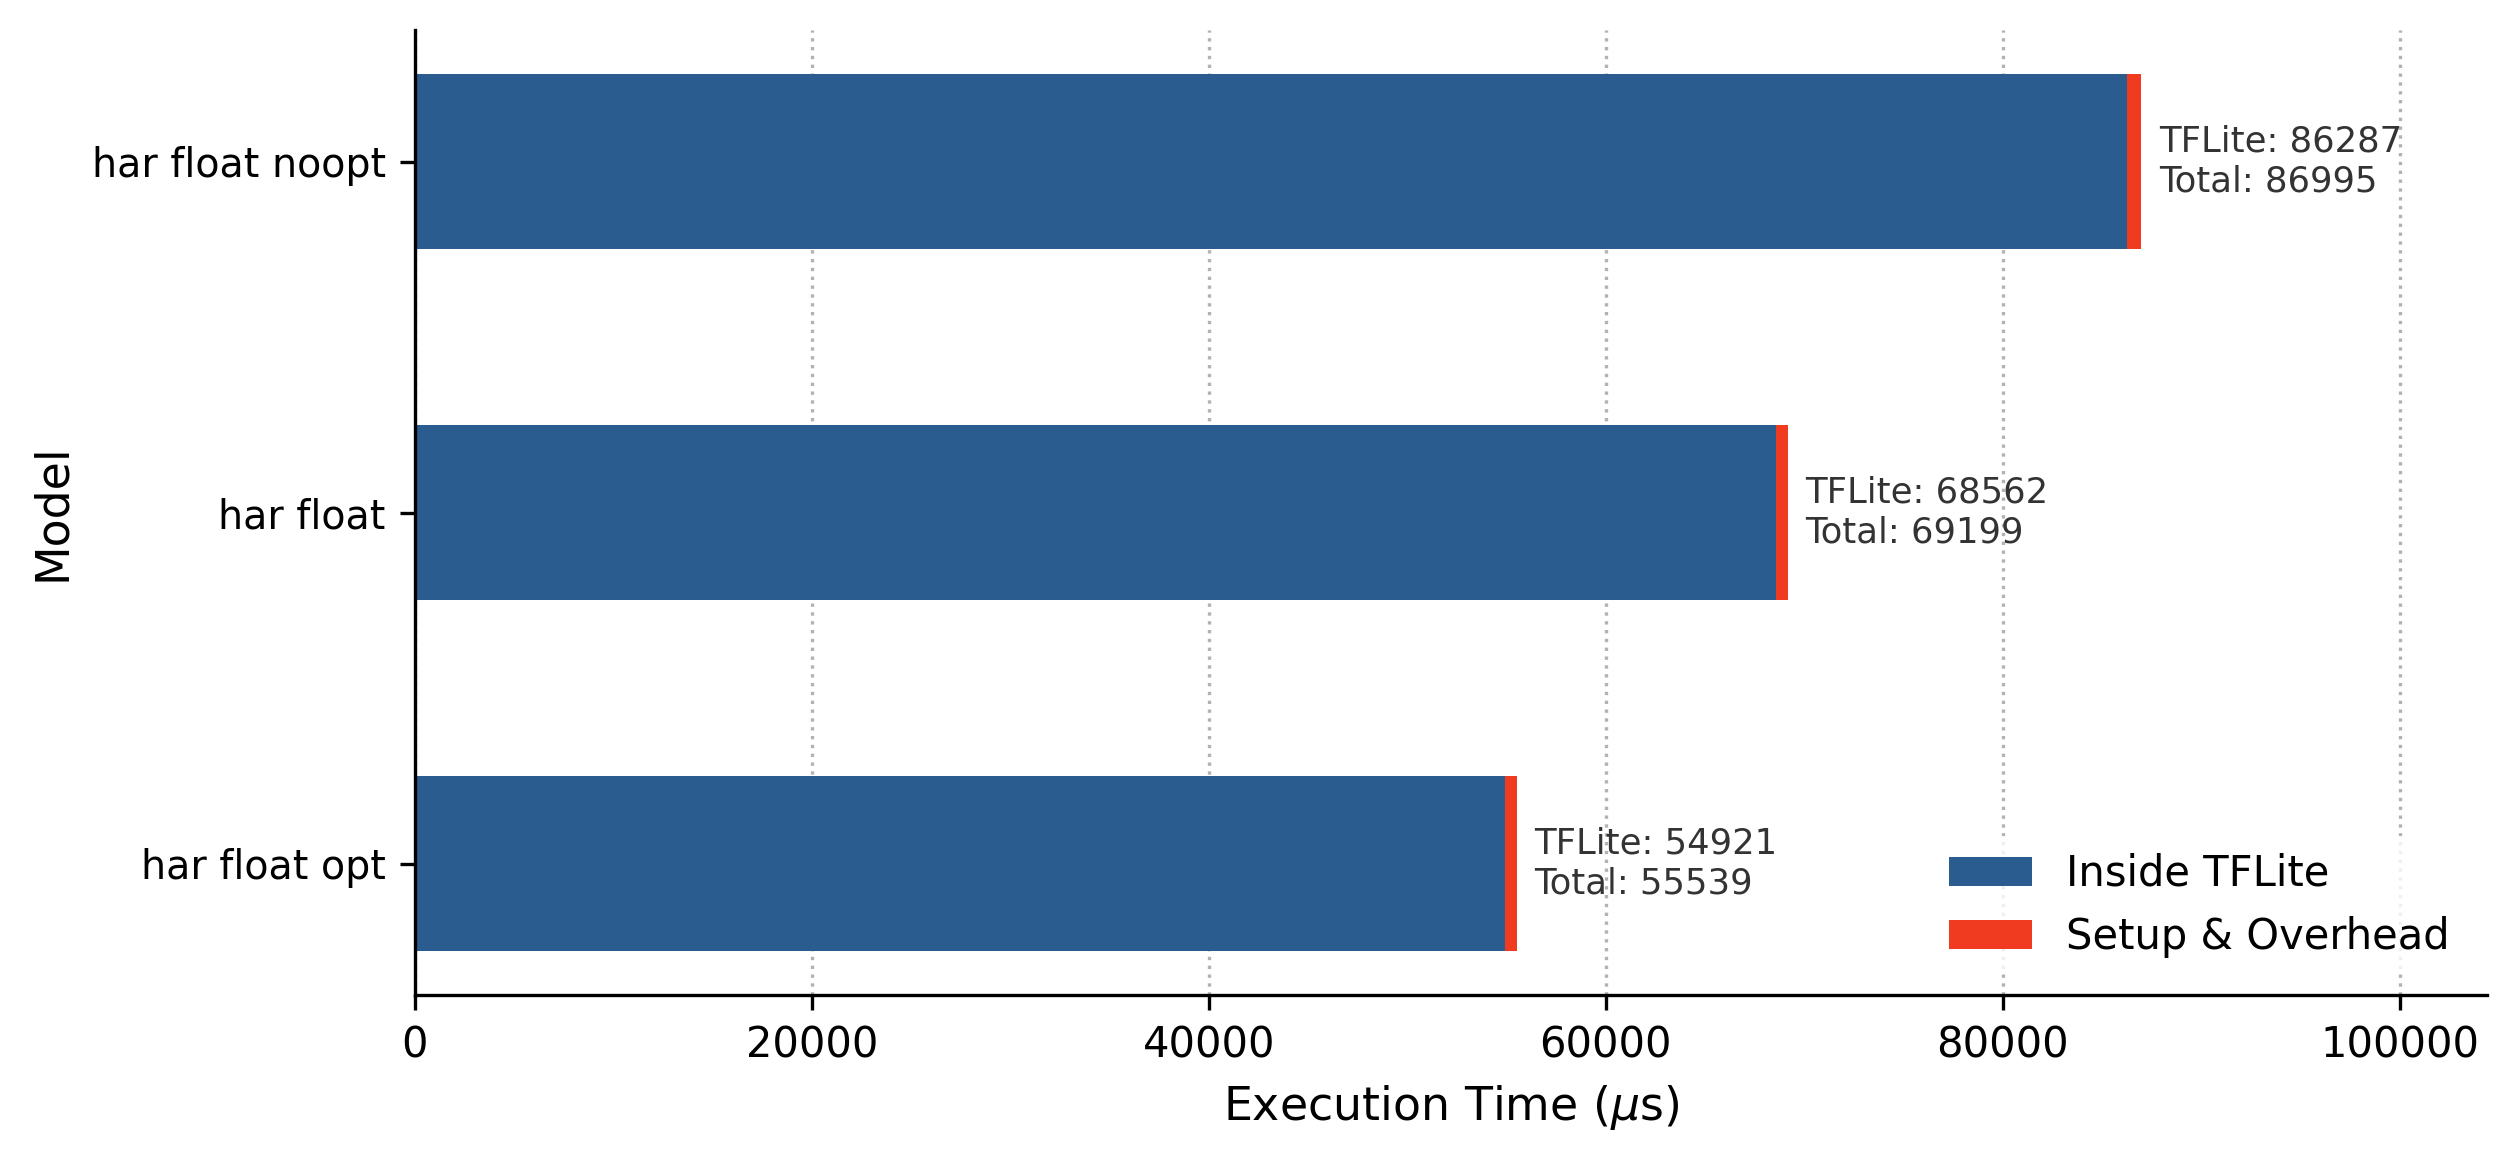
\includegraphics[width=\linewidth]{assets/result_figures/lat_har_float_opt.png}
  \caption{Execution latency across alternative levels of non-linear operation removal within the floating-point HAR architecture.}
  \label{fig:float_opt}
\end{figure}

The \textit{float} model variant achieved superior classification fidelity while bypassing expensive non-linear calculations. Conversely, the heavily optimized Euler discretization variant (\textit{float opt}) exhibited high variance and severe accuracy degradation when paired with subsequent quantization layers. Consequently, the \textit{float} configuration was chosen as our structural optimization baseline and was used for the remainder of experiments.

\begin{figure}[ht]
  \centering
  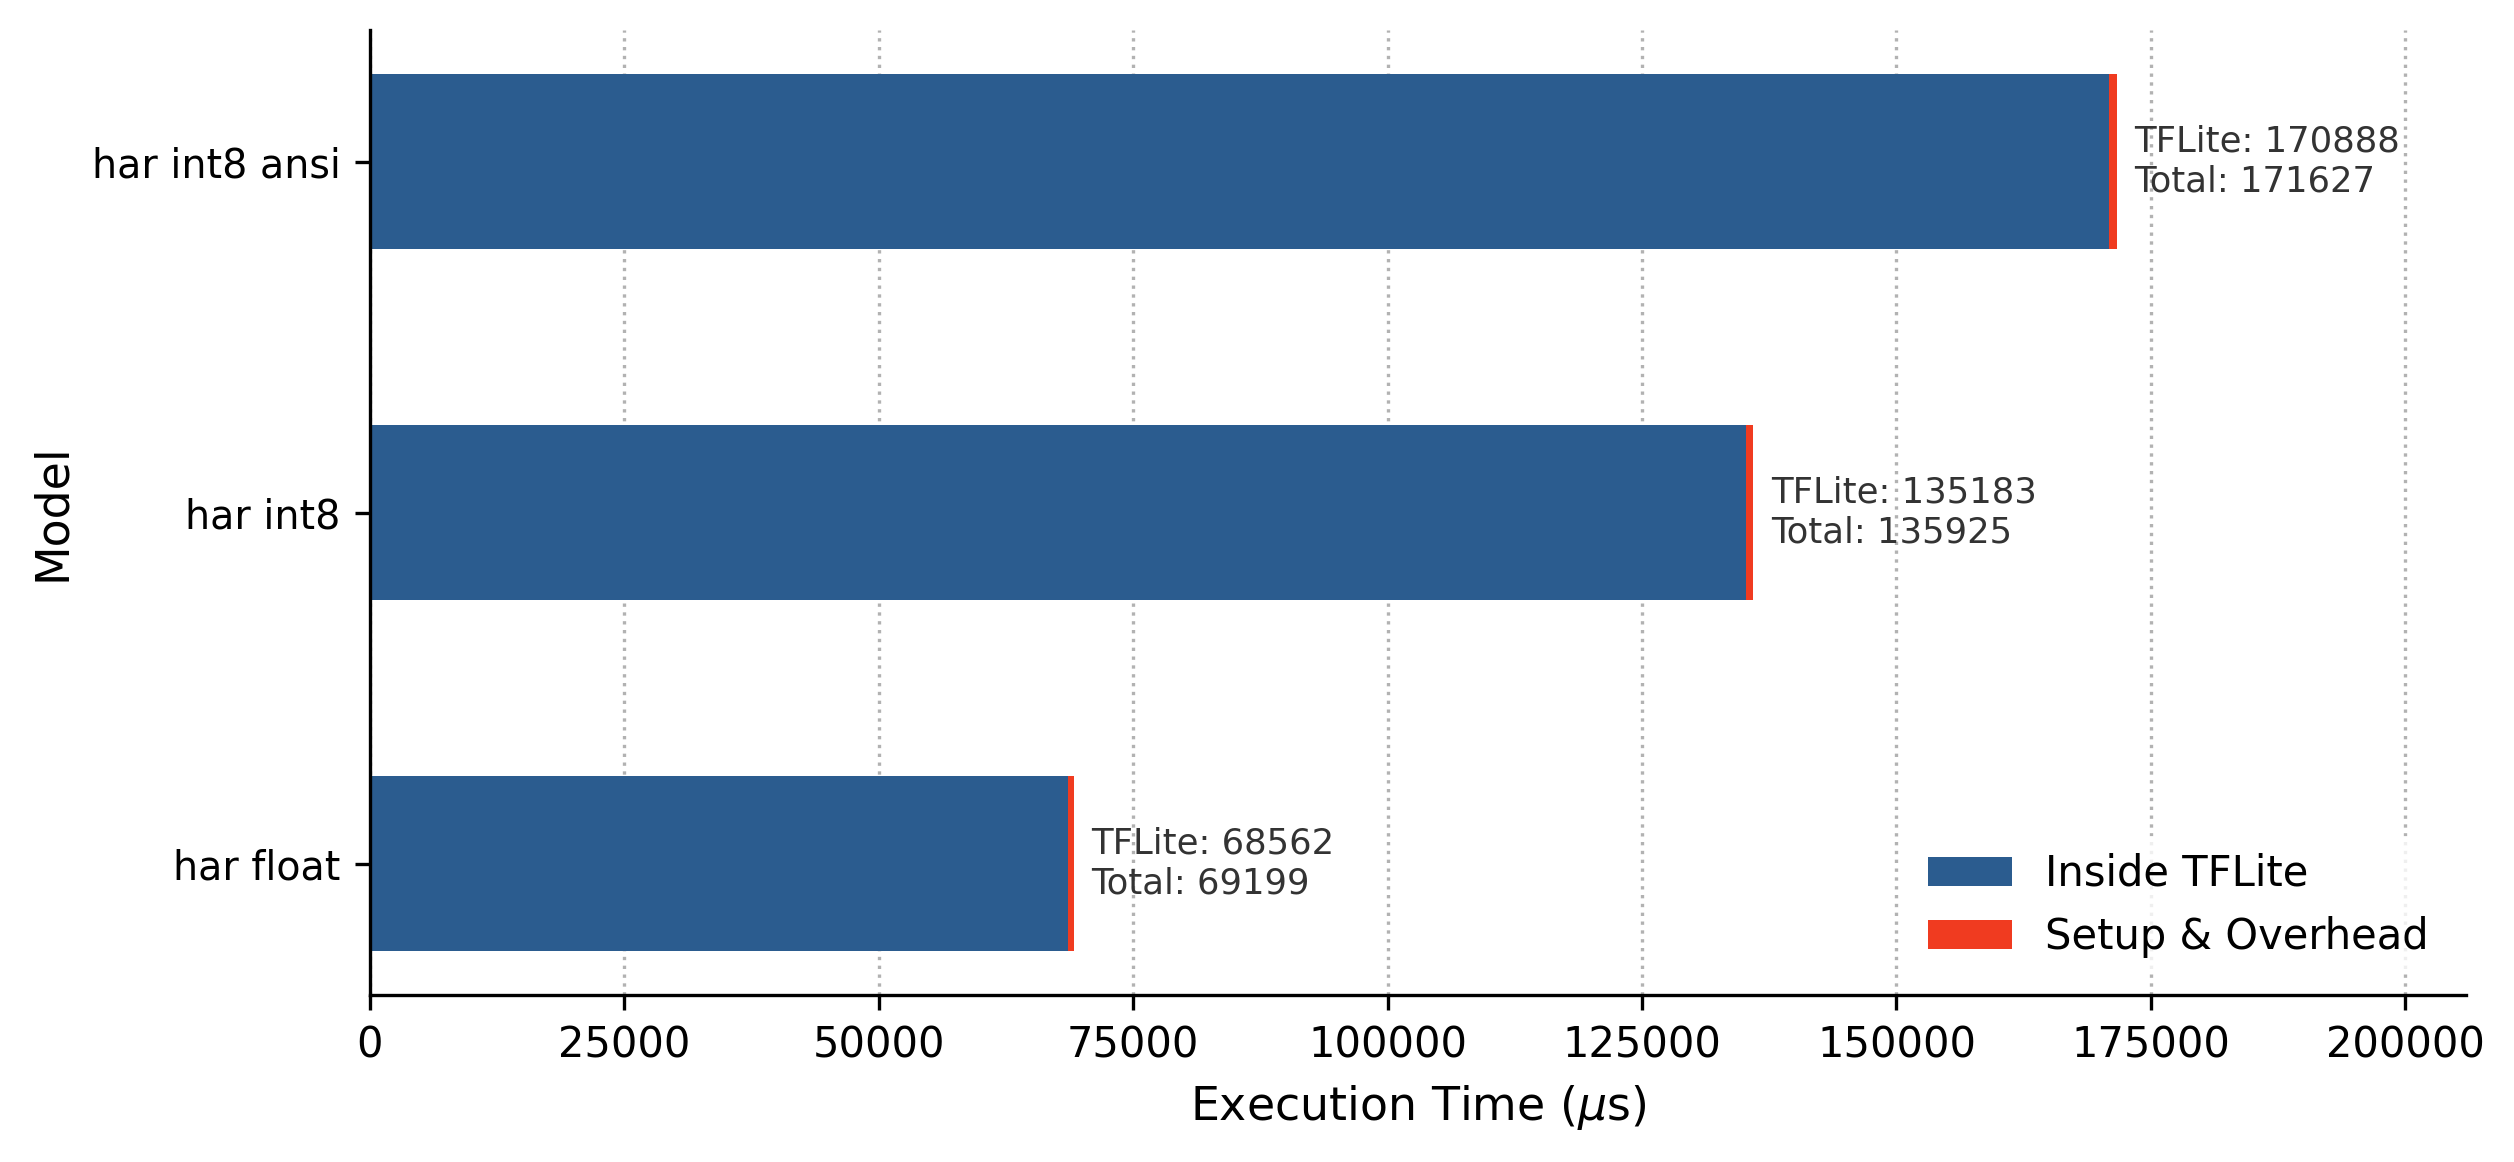
\includegraphics[width=\linewidth]{assets/result_figures/lat_har_datatypes.png}
  \caption{On-device execution latency comparisons for the unrolled HAR topology.}
  \label{fig:har_latency}
\end{figure}

A major finding of our on-device profiling is that the \texttt{INT8} quantized implementations are significantly slower than their \texttt{FLOAT32} equivalents, with integer execution times nearly doubling across identical layers (\autoref{fig:har_latency}). This counter-intuitive execution behavior is explained by the operation breakdown in \autoref{fig:operation_performance}. The runtime graph is completely dominated by element-wise multiplication (\texttt{MUL}) instructions. Although the ESP32-S3 contains hardware-level vector extensions capable of accelerating integer arithmetic, the standard, non-fused TFLM runtime infrastructure introduces extensive quantization/dequantization scaling and memory re-indexing overhead around every discrete scalar multiplication node. This software wrapper overhead ultimately overrides the raw clock-cycle efficiency of the integer execution unit.

Furthermore, platform optimization libraries demonstrated notable instability; activating vendor-specific \texttt{ESP\_NN} kernel accelerations caused measured accuracy on the HAR task to drop from 96\% to 56\%. Because this issue was strictly isolated to this specific layer graph, a separate baseline code path (INT8 ANSI) was profiled to isolate the compiler bug.

Finally, we evaluated the performance profiles of our proposed model-splitting design pattern against the standard unrolled paradigm (\autoref{fig:final_latency}). Splitting the model introduces a massive latency penalty, directly multiplying overall execution duration. This overhead is fundamentally external to the TFLM interpreter kernel itself; it is driven by host-side memory orchestration, where data pointers must be manually copied, reshuffled, and verified across three separate sub-graph interfaces at every consecutive time step.

\begin{figure}[ht]
  \centering
  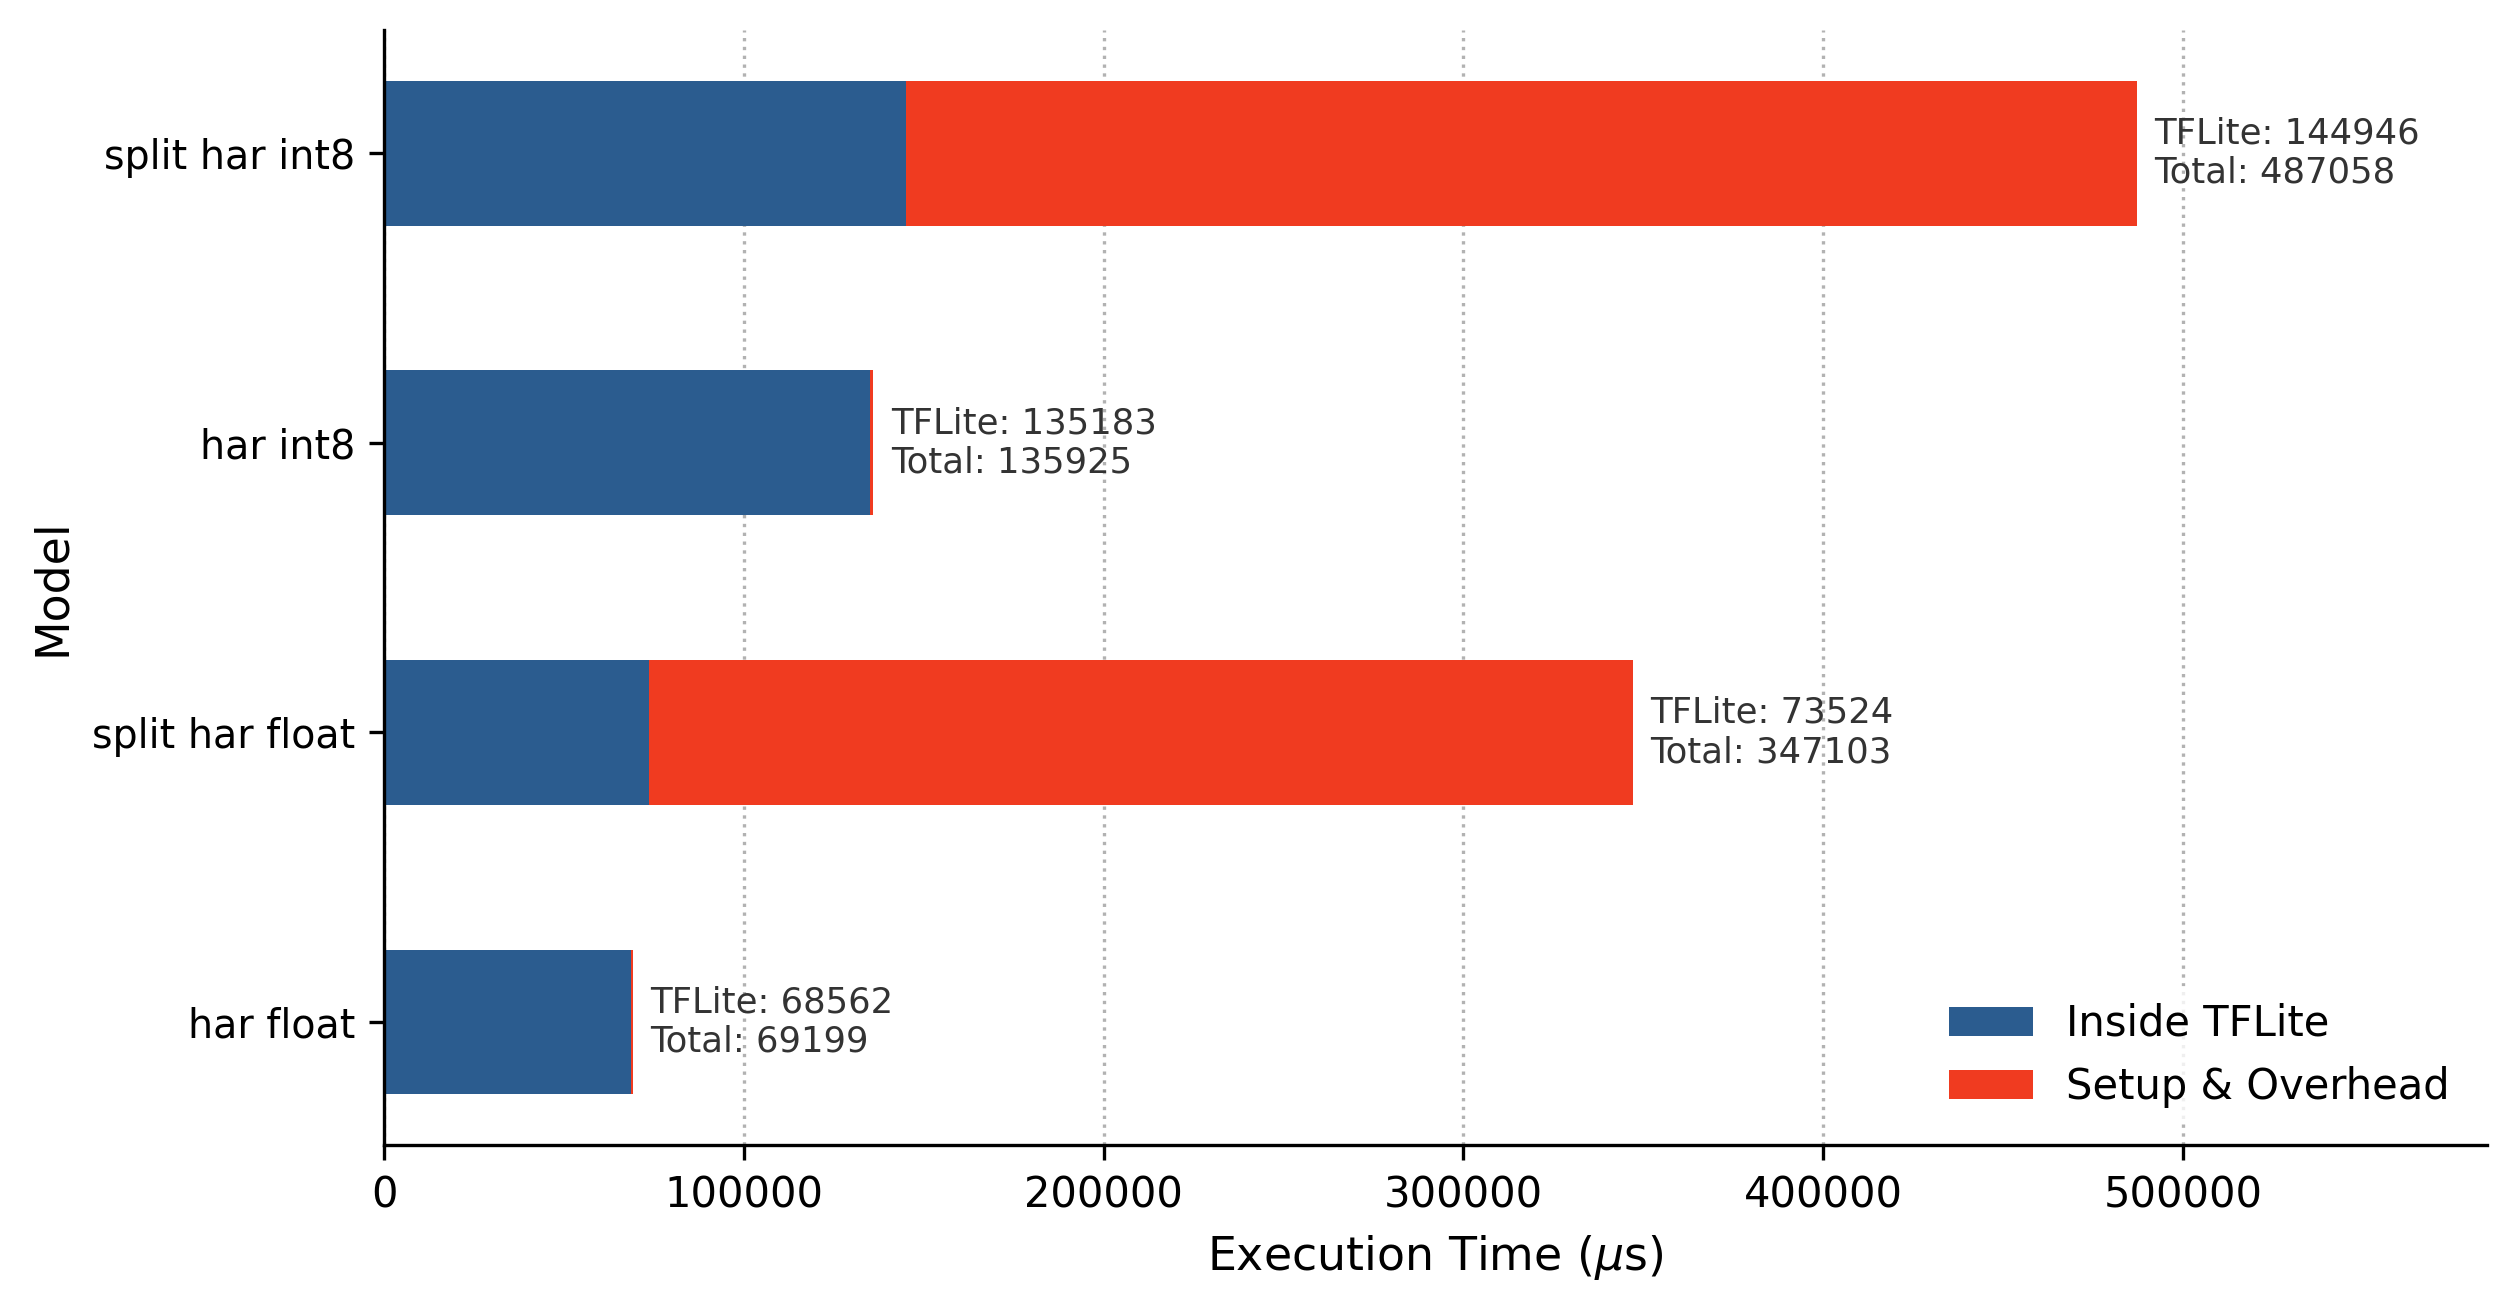
\includegraphics[width=\linewidth]{assets/result_figures/lat_har_vs_split.png}
  \vspace{0.75em}
  \\{\small (a) Latency comparison between unrolled and split HAR configurations.}

  \medskip
  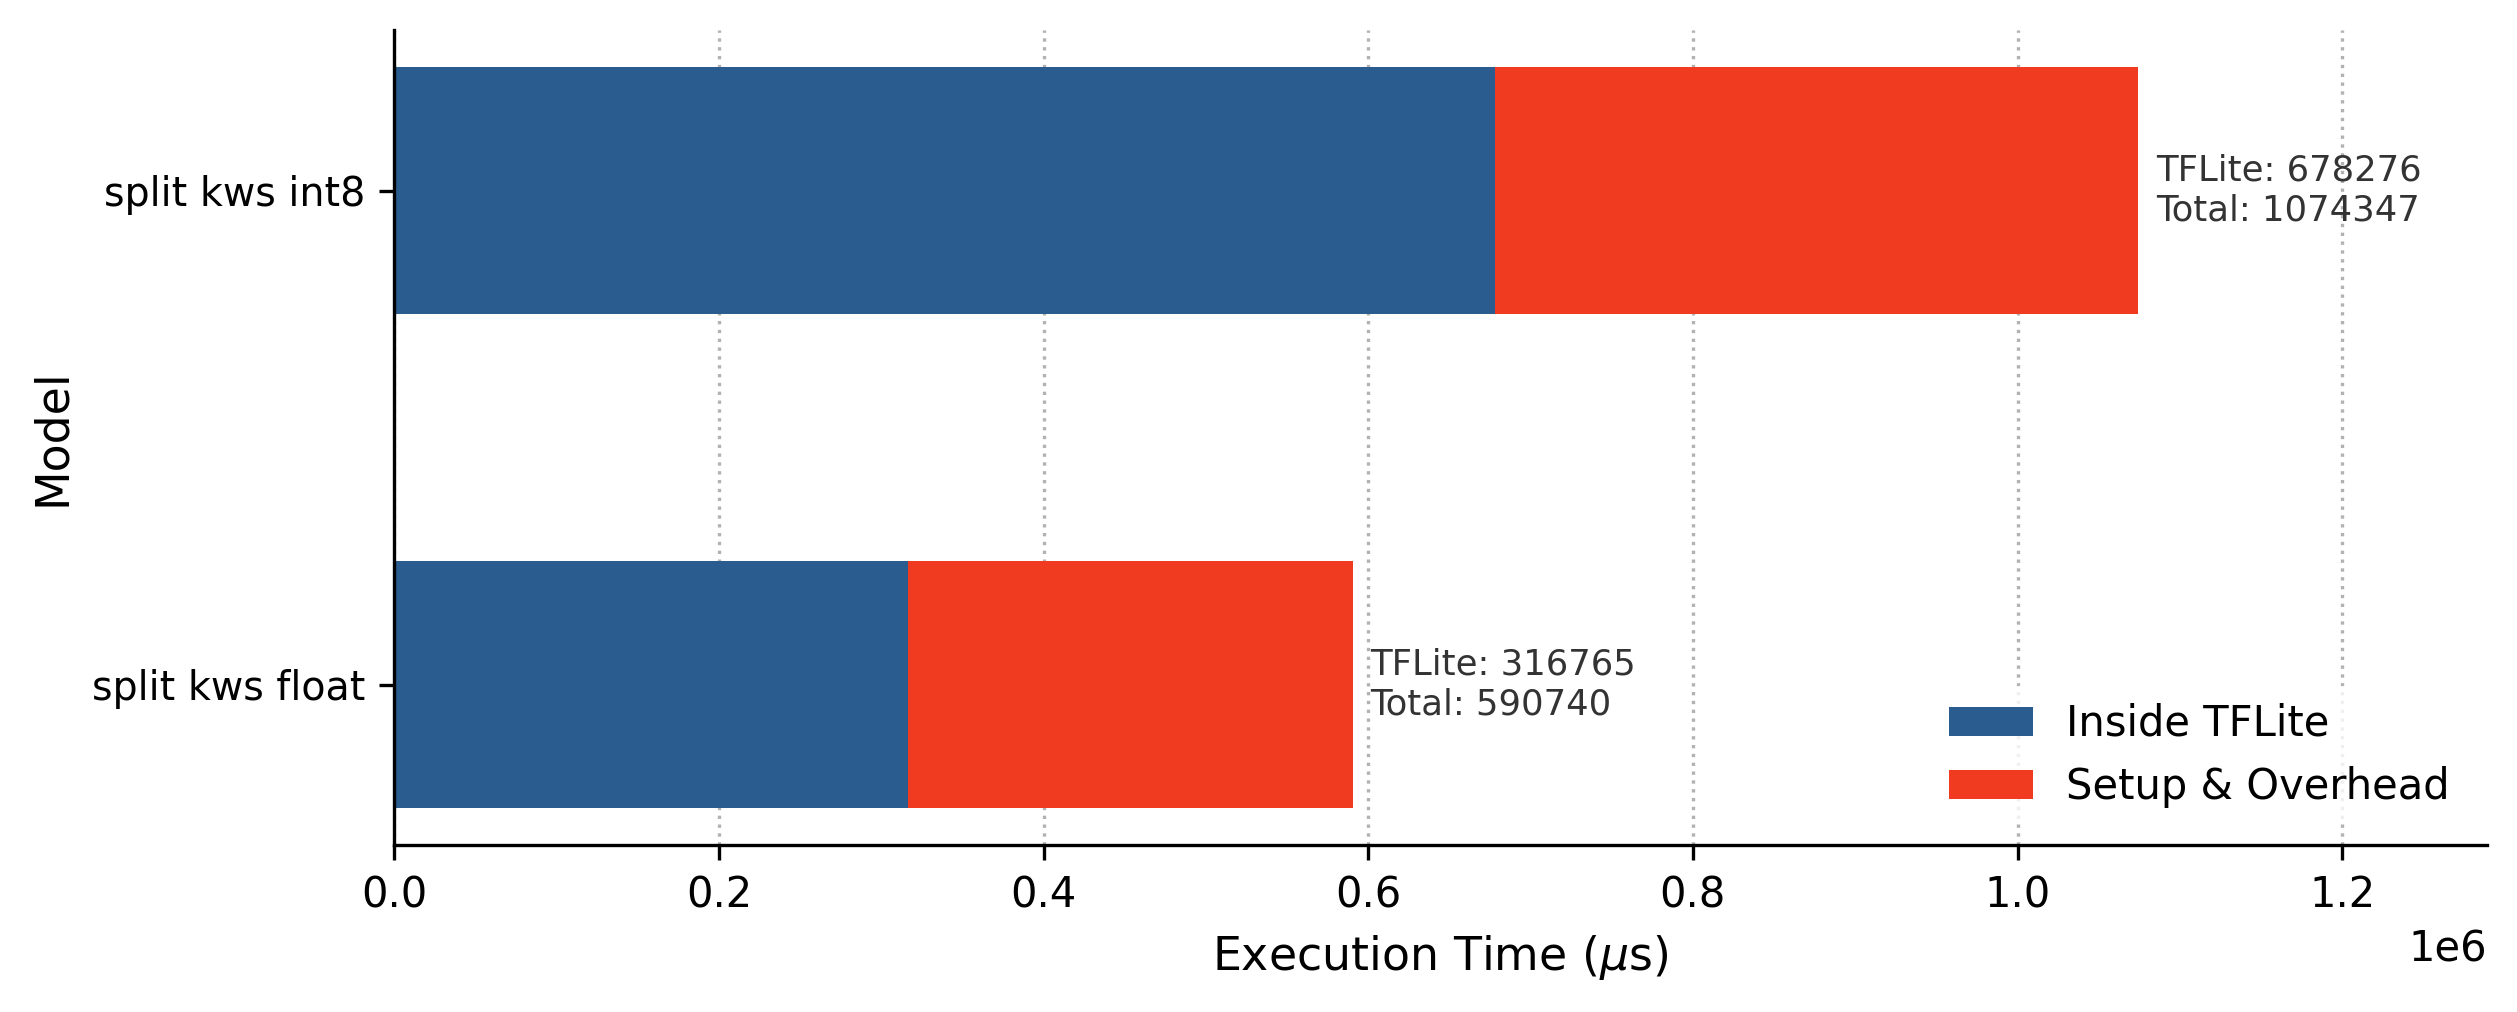
\includegraphics[width=\linewidth]{assets/result_figures/lat_kws_split.png}
  \vspace{0.75em}
  \\{\small (b) Latency profile of the partitioned KWS architecture.}
  \caption{Detailed latency benchmarks across isolated microcontroller execution strategies.}
  \label{fig:final_latency}
\end{figure}

\begin{figure*}[ht]
  \centering
  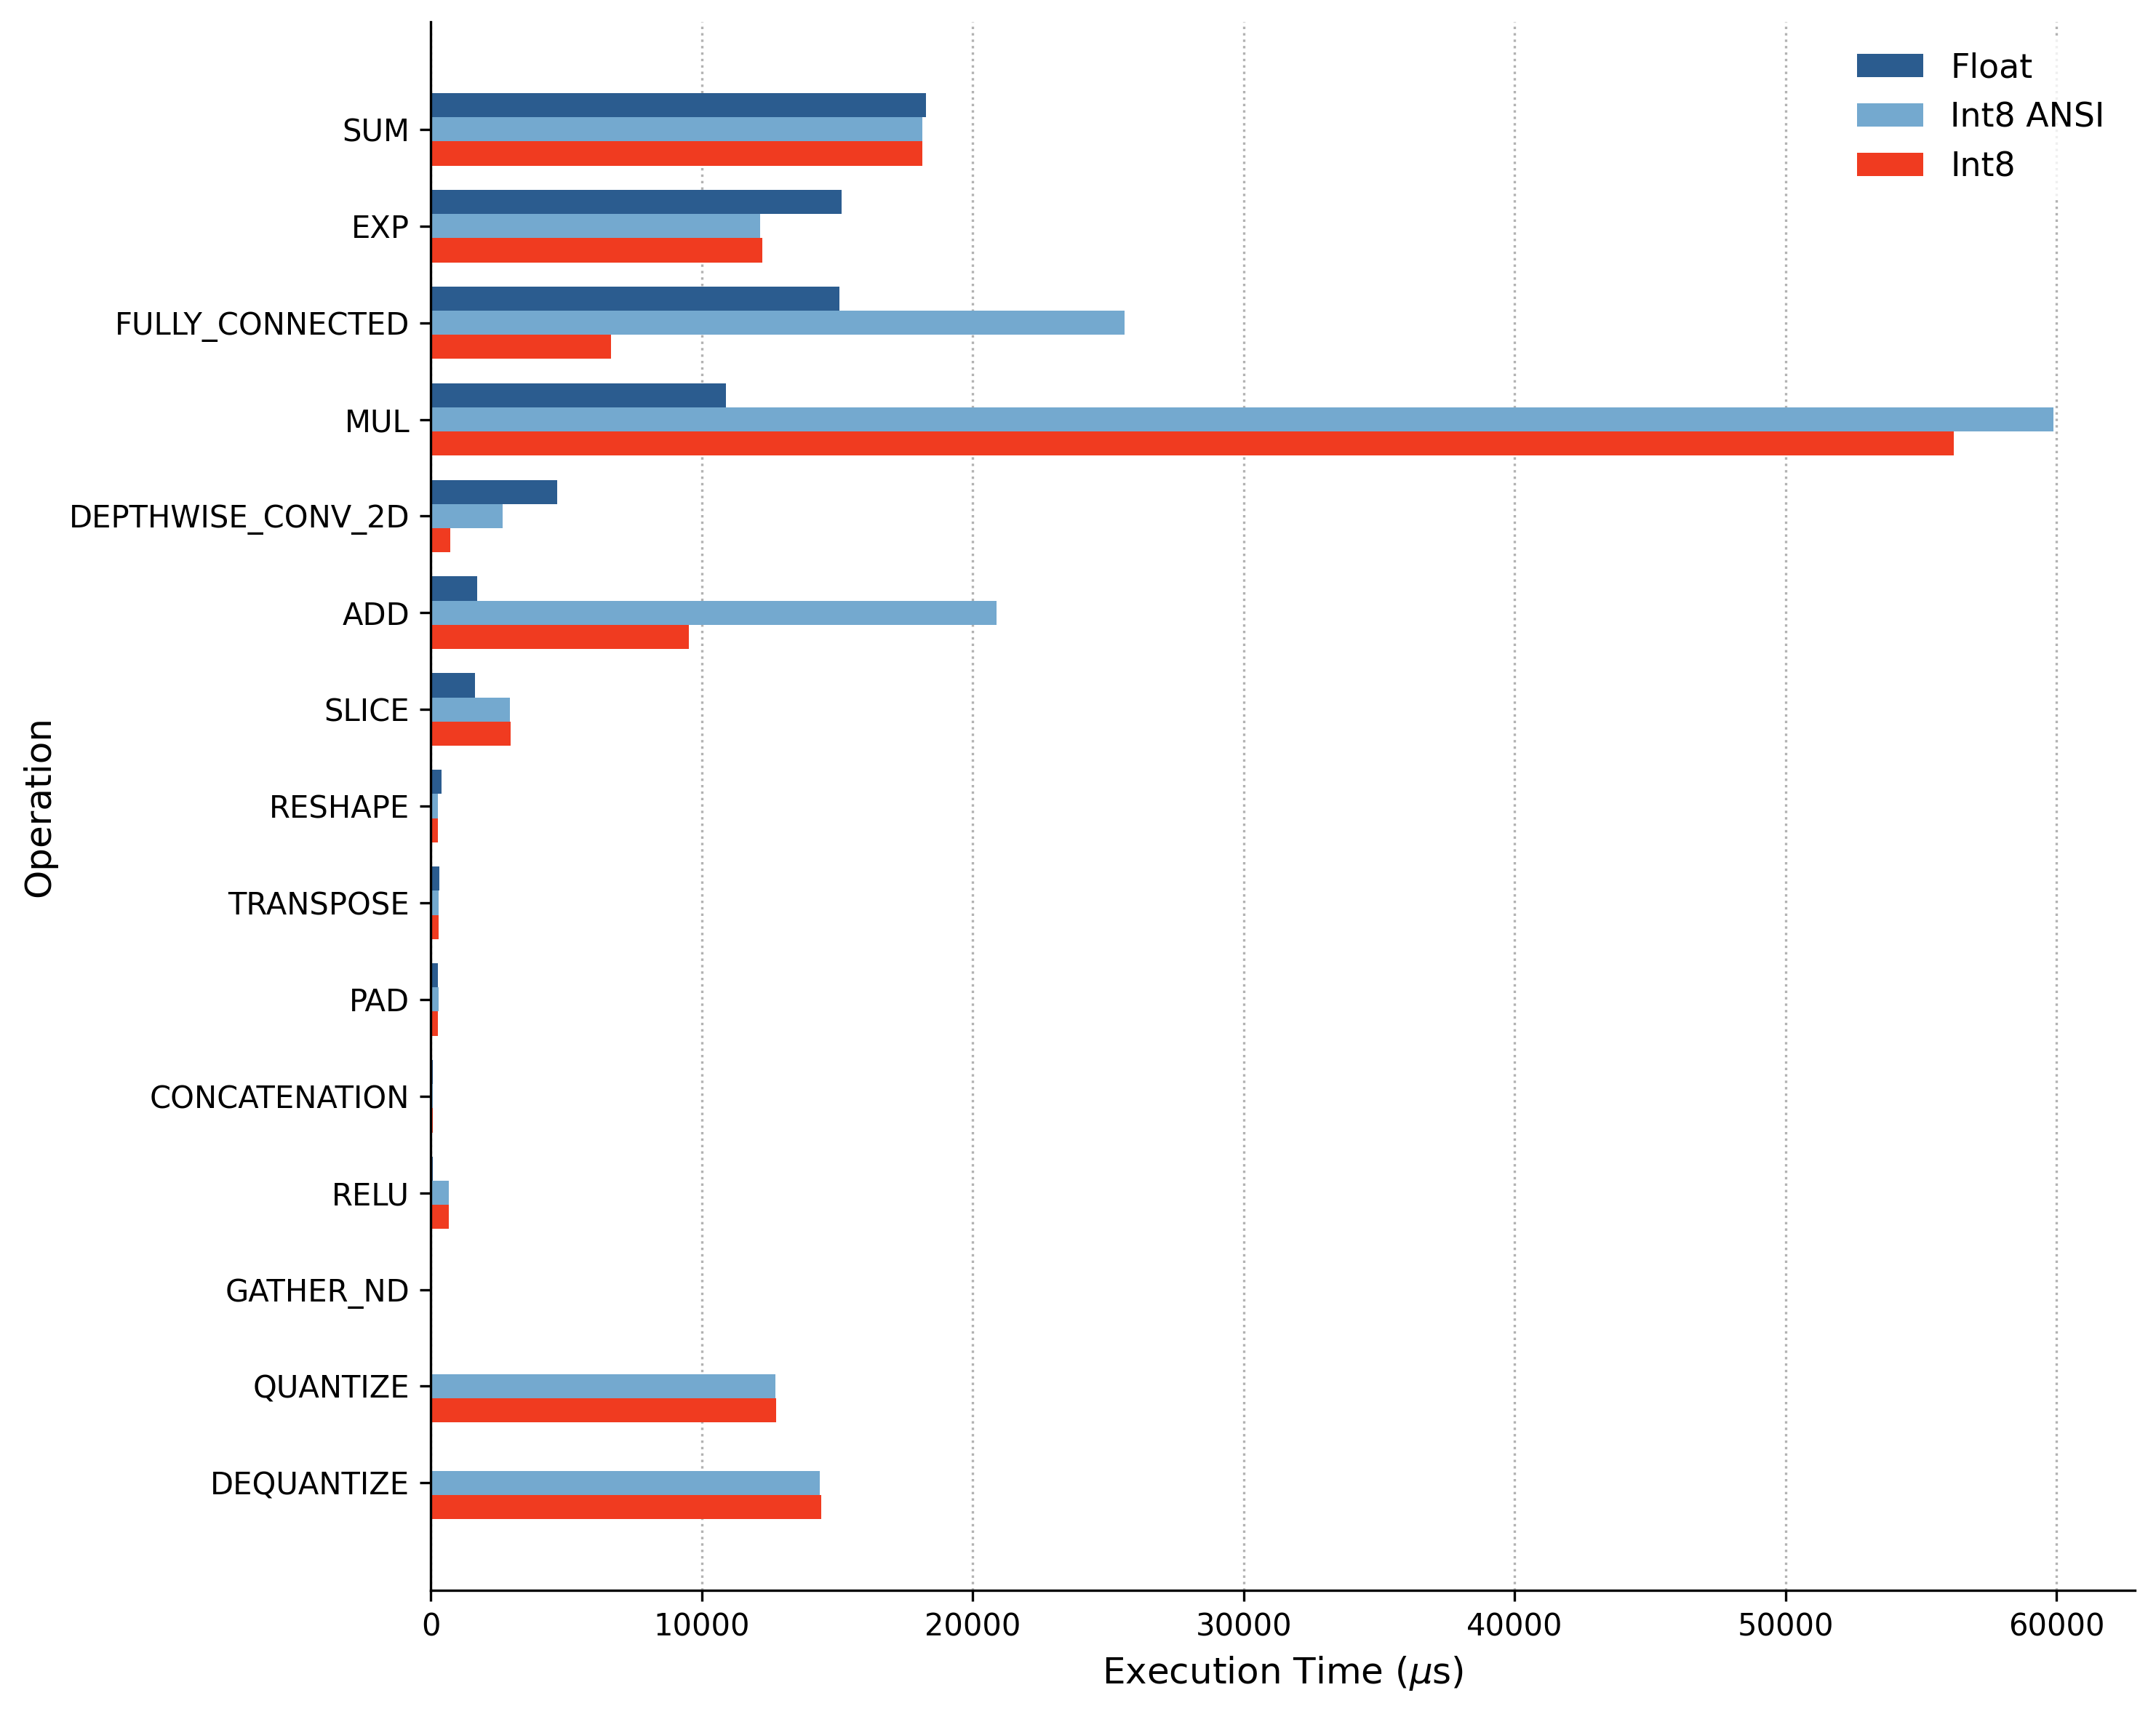
\includegraphics[width=0.7\textwidth]{assets/result_figures/operation_performance_linear.png}
  \caption{Granular execution impact per instruction type across Float, INT8 ANSI, and INT8 HAR configurations.}
  \label{fig:operation_performance}
\end{figure*}

While splitting the graph incurs a substantial speed penalty, it successfully addresses memory bottlenecks. Volatile memory usage behaves predictably: INT8 variants demand significantly smaller heap allocations (\autoref{fig:memory}).

Crucially, the loop-partitioned model reduces peak working RAM allocations relative to the unrolled network, despite requiring additional static data buffers to manually bridge the sub-graph interfaces. The specific scaling dynamics of these intermediate transfer matrices vary linearly based on input tensor dimensions (\autoref{fig:kws_memory}).

\begin{figure}[ht]
  \centering
  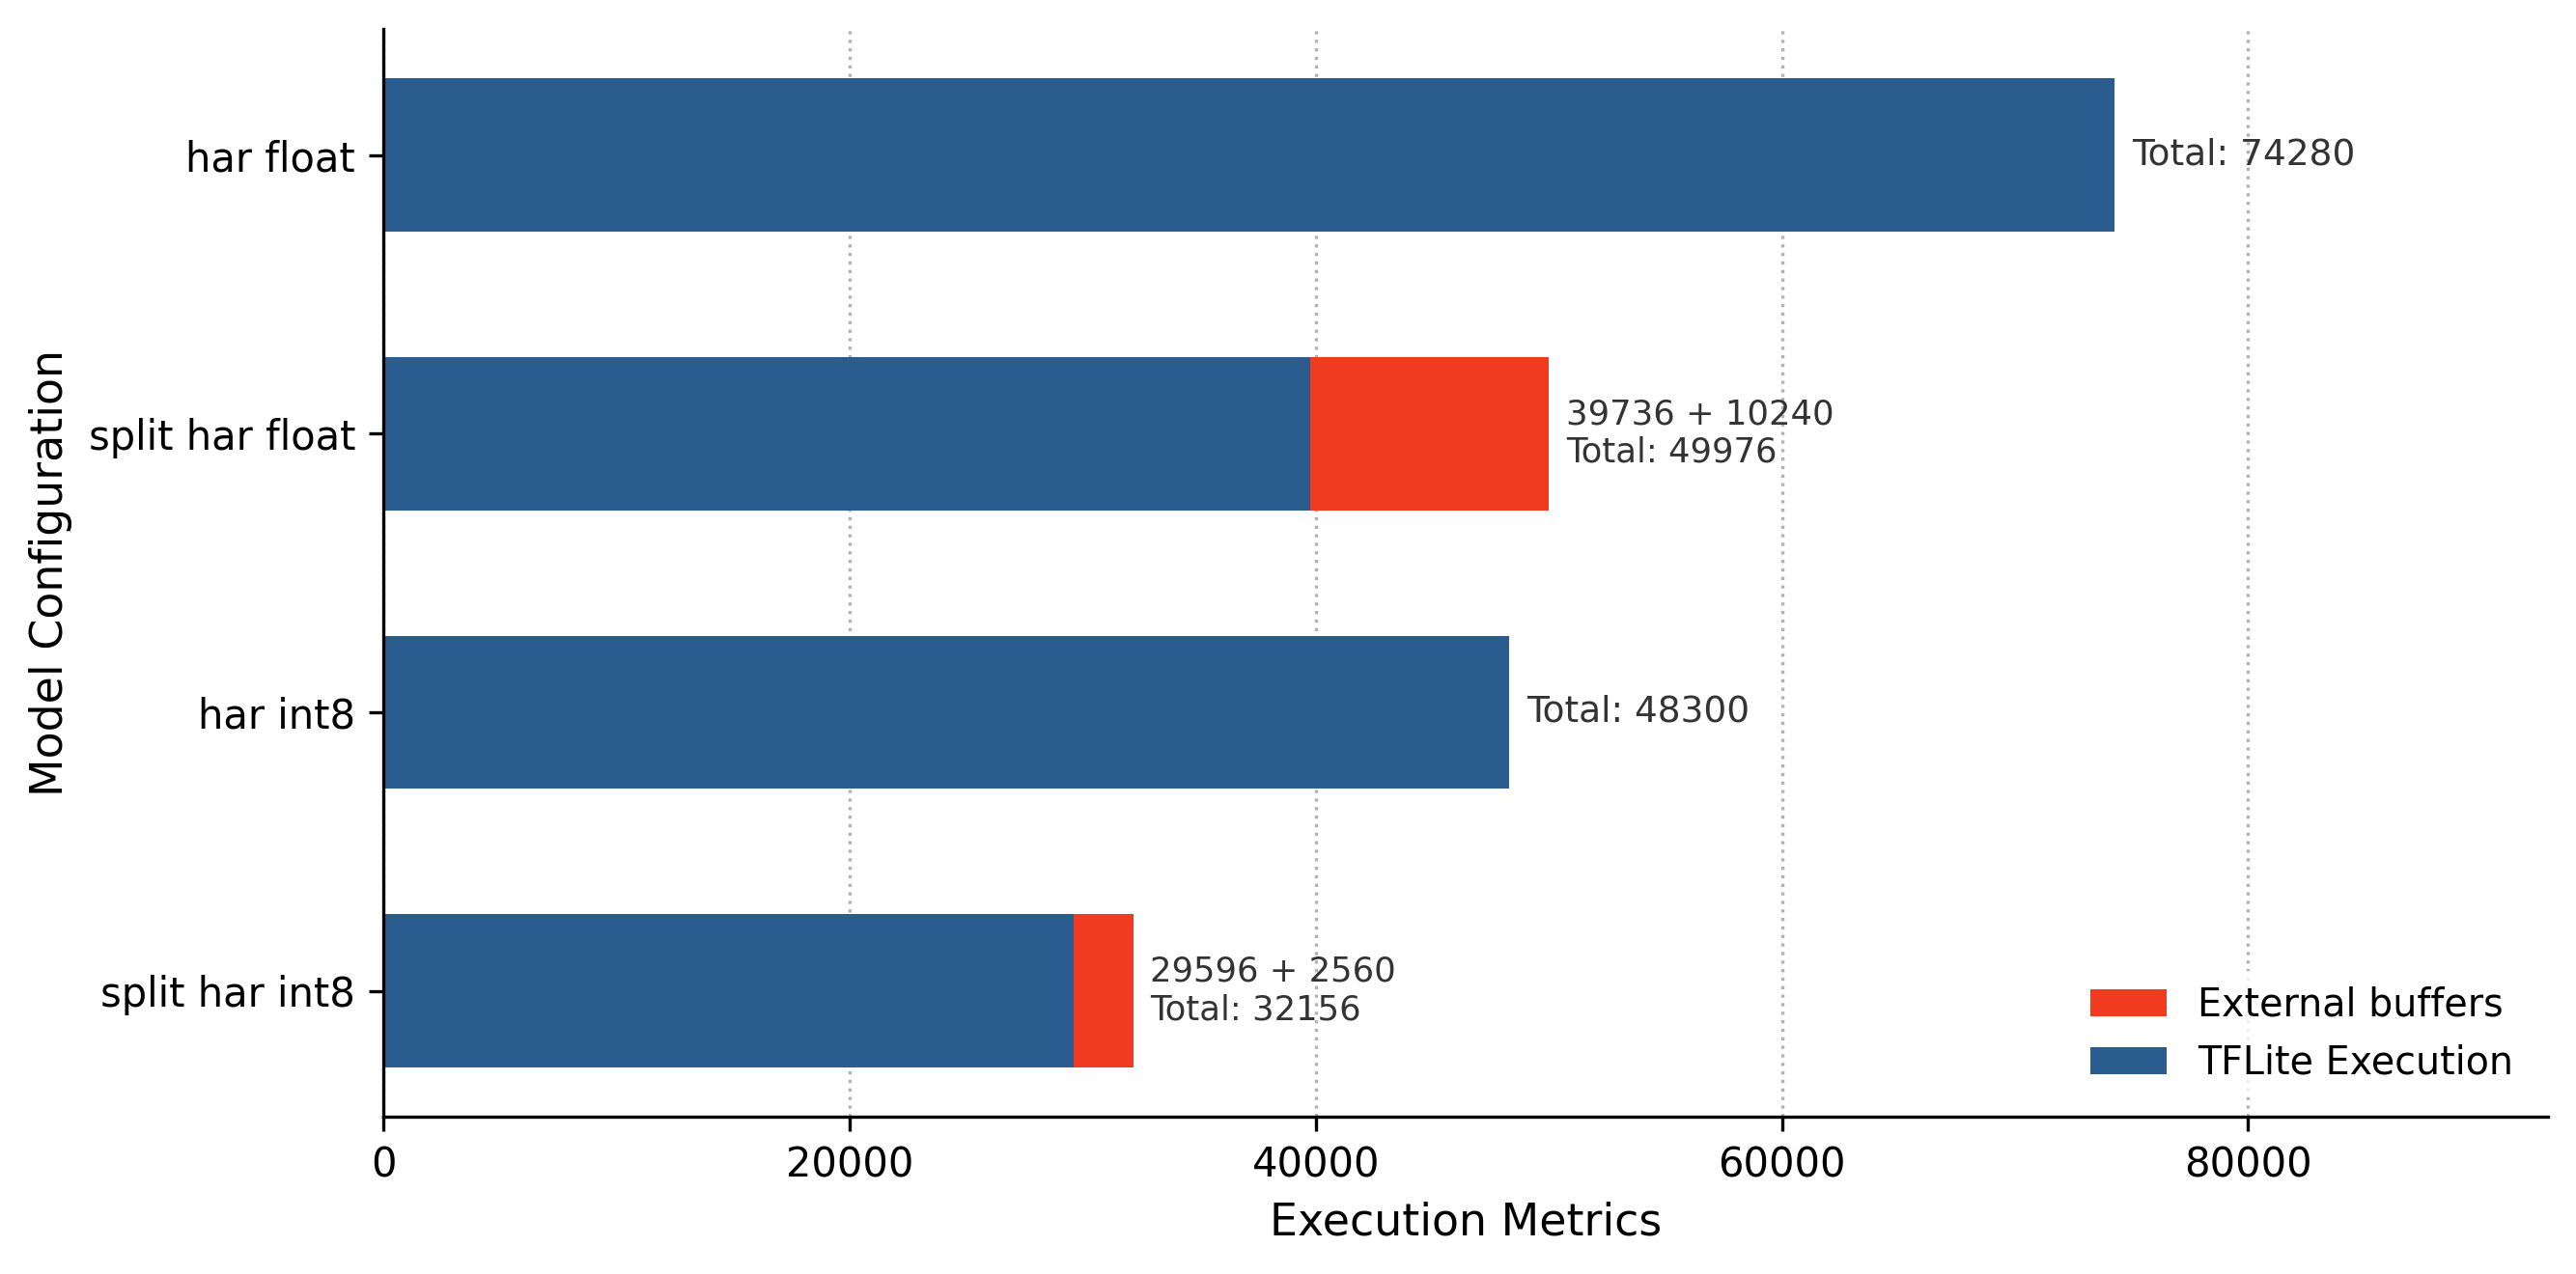
\includegraphics[width=\linewidth]{assets/result_figures/mem_all_har_combined.png}
  \caption{Peak working RAM consumption across alternative HAR model formats.}
  \label{fig:memory}
\end{figure}

\begin{figure}[ht]
  \centering
  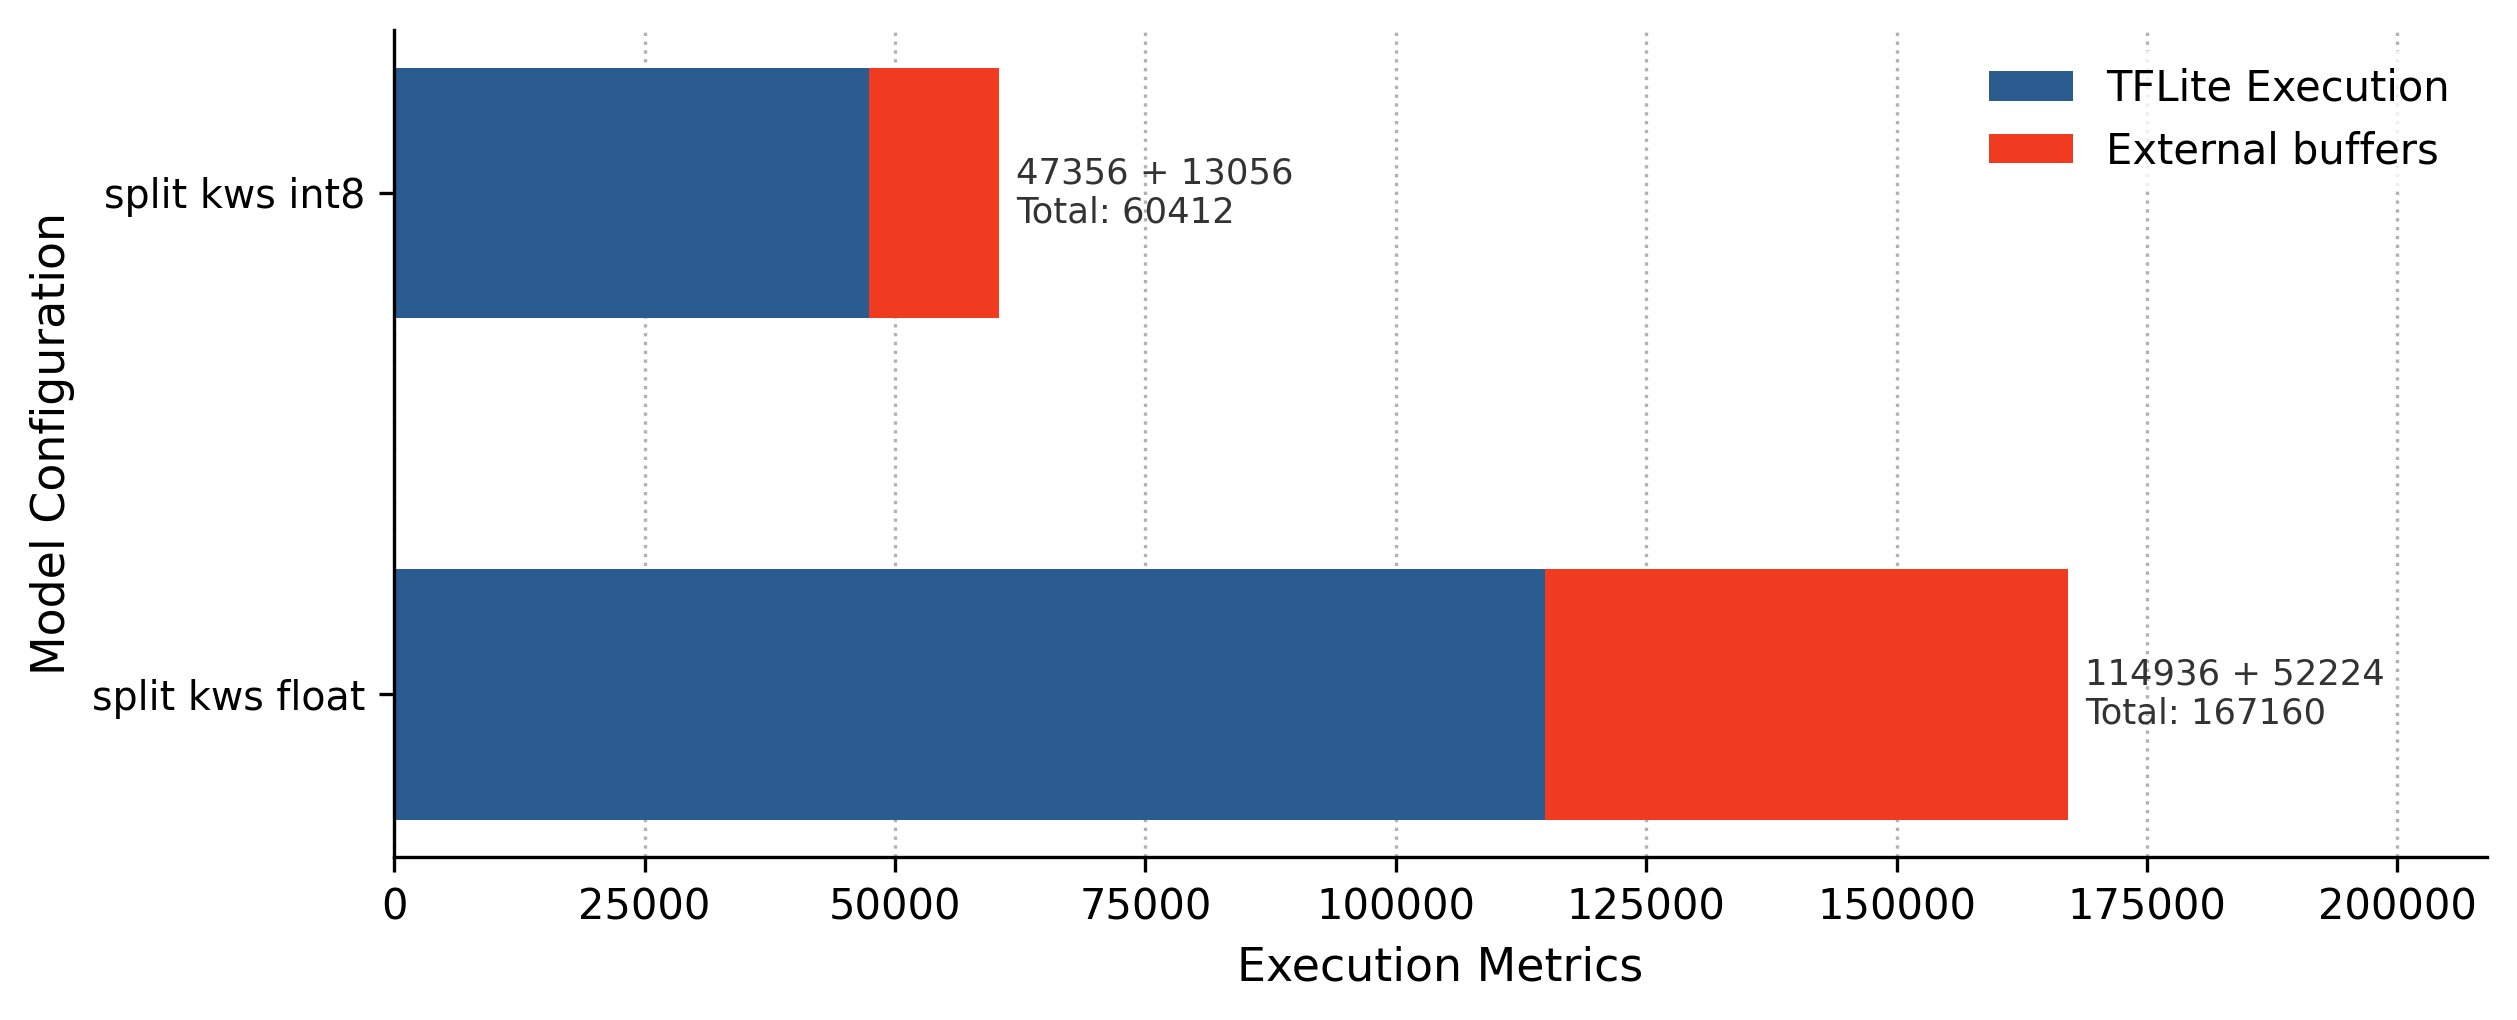
\includegraphics[width=\linewidth]{assets/result_figures/mem_split_kws.png}
  \caption{Peak working RAM allocations mapped across varying KWS sequence dimensions.}
  \label{fig:kws_memory}
\end{figure}
